%DIF 1-3c1-3
%DIF LATEXDIFF DIFFERENCE FILE
%DIF DEL ../oro-cs-seminar.tex       Mon Mar 25 14:20:53 2019
%DIF ADD oro-cs-seminar.jorden.tex   Mon Mar 25 17:40:36 2019
%DIF < \RequirePackage[]{silence}
%DIF < \WarningFilter{latex}{Marginpar on page}
%DIF < \WarningFilter{lcg}{Using an already existing counter rand}
%DIF -------
\RequirePackage[]{silence} \WarningFilter{latex}{Marginpar %DIF > 
on page} \WarningFilter{lcg}{Using an already existing %DIF > 
counter rand} %DIF > 
%DIF -------
\documentclass[article, oneside]{aaltoseries}
\usepackage[utf8]{inputenc}
\usepackage[english]{babel}
\usepackage{IEEEtrantools}
\usepackage[hyphens]{url} % allow hyphens to break urls
\Urlmuskip=0mu  plus 1mu % allow for some spacing inside urls
\usepackage[hidelinks]{hyperref}
\usepackage[acronym]{glossaries}
\usepackage{amsfonts}
\usepackage{todonotes}
\usepackage[normalem]{ulem}
\usepackage{xcolor}
\usepackage{xspace}
\usepackage{textcomp}
\usepackage{etoolbox}
\usepackage[numbers]{natbib}
%DIF 20a20
\usepackage{enumitem} %DIF > 
%DIF -------
\newcommand{\TODO}[1]{\todo[inline]{#1}}
\newcommand{\jwnote}[1]{\todo[size=\small,color=blue!40]{#1}}
\newcommand{\JWNOTE}[1]{\todo[size=\small,inline,color=blue!40]{#1}}
\newcommand{\modif}[1]{\textcolor{blue}{#1}}
\newcommand\remove{\bgroup\markoverwith
{\textcolor{red}{\rule[0.5ex]{2pt}{0.8pt}}}\ULon}
\newcommand{\discuss}[1]{\todo[size=\small,color=green!40]{#1}}

%DIF 28-31c29-34
%DIF < \geometry{left=4cm,right=4cm,marginparwidth=3.5cm,marginparsep=5mm} % TODO: remove
%DIF < % \geometry{left=1cm,right=7cm,marginparwidth=6.5cm,marginparsep=5mm} % TODO: remove
%DIF < % \reversemarginpar % for todo notes on the wider side
%DIF < % \geometry{marginparwidth=5cm,marginparsep=3mm} % TODO: remove
%DIF -------
\geometry{left=4cm,right=4cm,marginparwidth=3.5cm,marginparsep=5mm} %DIF > 
% TODO: remove %DIF > 
% \geometry{left=1cm,right=7cm,marginparwidth=6.5cm,marginparsep=5mm} %DIF > 
% % TODO: remove \reversemarginpar % for todo notes on the %DIF > 
% wider side \geometry{marginparwidth=5cm,marginparsep=3mm} %DIF > 
% % TODO: remove %DIF > 
%DIF -------

% Use “\tocite{}” to get “citation needed” in document
\newcommand\tocite[1]{
	\todo{\ifstrempty{#1}{Citation needed}{#1}}
%DIF 36-37c39
%DIF < 	[\,\textbf{\color{red}!}\,]
%DIF < }
%DIF -------
	[\,\textbf{\color{red}!}\,]} %DIF > 
%DIF -------


%DIF 40c42-43
%DIF < % ************************ Custom Referencing **********************************
%DIF -------
% ************************ Custom Referencing %DIF > 
% ********************************** %DIF > 
%DIF -------
\newcommand{\Fref}[1]{Figure~\ref{#1}}
\newcommand{\fref}[1]{figure~\ref{#1}}
\newcommand{\Tref}[1]{Table~\ref{#1}}
\newcommand{\tref}[1]{table~\ref{#1}}
\newcommand{\Eref}[1]{Equation~\ref{#1}}
\newcommand{\eref}[1]{equation~\ref{#1}}
\newcommand{\Sref}[1]{Section~\ref{#1}}
\newcommand{\sref}[1]{section~\ref{#1}}
\newcommand{\Lref}[1]{Listing~\ref{#1}}
\newcommand{\lref}[1]{listing~\ref{#1}}


\newcommand{\app}[1]{A\textsc{pp}$_{#1}$\xspace}

\glsenableentrycount
%DIF 56-59c59-60
%DIF < \renewcommand\gls\cgls
%DIF < \renewcommand\glspl\cglspl
%DIF < \renewcommand\Gls\cGls
%DIF < \renewcommand\Glspl\cGlspl
%DIF -------
\renewcommand\gls\cgls \renewcommand\glspl\cglspl %DIF > 
\renewcommand\Gls\cGls \renewcommand\Glspl\cGlspl %DIF > 
%DIF -------
\newacronym{os}{OS}{operating system}
\newacronym{vm}{VM}{virtual machine}
%DIF 62a63
\newacronym{pha}{PHA}{potentially harmful applications} %DIF > 
%DIF -------

\title{Android App Collusion}


\author{Ervin Oro% Your first and last name: do _not_ add your student number
\\\textnormal{\texttt{ervin.oro@aalto.fi}}} % Your Aalto e-mail address
\affiliation{\textbf{Tutor}: Jorden Whitefield} % First and last name of your tutor

%==========================================================
%DIF PREAMBLE EXTENSION ADDED BY LATEXDIFF
%DIF UNDERLINE PREAMBLE %DIF PREAMBLE
\RequirePackage[normalem]{ulem} %DIF PREAMBLE
\RequirePackage{color}\definecolor{RED}{rgb}{1,0,0}\definecolor{BLUE}{rgb}{0,0,1} %DIF PREAMBLE
\providecommand{\DIFaddtex}[1]{{\protect\color{blue}\uwave{#1}}} %DIF PREAMBLE
\providecommand{\DIFdeltex}[1]{{\protect\color{red}\sout{#1}}}                      %DIF PREAMBLE
%DIF SAFE PREAMBLE %DIF PREAMBLE
\providecommand{\DIFaddbegin}{} %DIF PREAMBLE
\providecommand{\DIFaddend}{} %DIF PREAMBLE
\providecommand{\DIFdelbegin}{} %DIF PREAMBLE
\providecommand{\DIFdelend}{} %DIF PREAMBLE
%DIF FLOATSAFE PREAMBLE %DIF PREAMBLE
\providecommand{\DIFaddFL}[1]{\DIFadd{#1}} %DIF PREAMBLE
\providecommand{\DIFdelFL}[1]{\DIFdel{#1}} %DIF PREAMBLE
\providecommand{\DIFaddbeginFL}{} %DIF PREAMBLE
\providecommand{\DIFaddendFL}{} %DIF PREAMBLE
\providecommand{\DIFdelbeginFL}{} %DIF PREAMBLE
\providecommand{\DIFdelendFL}{} %DIF PREAMBLE
%DIF HYPERREF PREAMBLE %DIF PREAMBLE
\providecommand{\DIFadd}[1]{\texorpdfstring{\DIFaddtex{#1}}{#1}} %DIF PREAMBLE
\providecommand{\DIFdel}[1]{\texorpdfstring{\DIFdeltex{#1}}{}} %DIF PREAMBLE
%DIF END PREAMBLE EXTENSION ADDED BY LATEXDIFF

\begin{document}
\bstctlcite{BSTcontrol}

\maketitle
\todo{set proper margins and document format}
%==========================================================

\begin{abstract}
\TODO{abstract}

\vspace{3mm}
\noindent KEYWORDS: \todo[inline, inlinewidth=5cm, noinlinepar]{list, of, key, words}

\end{abstract}

%============================================================

\section{Introduction}
\label{sec:intro}
\DIFdelbegin %DIFDELCMD < 

%DIFDELCMD < %%%
\DIFdel{Android is an \mbox{%DIFAUXCMD
\gls{os}}\hspace{0pt}%DIFAUXCMD
that }\DIFdelend %DIF > 
\DIFaddbegin \DIFadd{The number and complexity of attacks against mobile devices
are increasing~\mbox{%DIFAUXCMD
\cite{AOSP,AVTESTGH2018}}\hspace{0pt}%DIFAUXCMD
. There is cause for
concern since mobiles are rich sources of data, and the data
is of interest to many malicious and benign entities. Mobile
Malware is software that is designed to gain unauthorised
access to data on the device, disrupt, or cause damage.
\mbox{%DIFAUXCMD
\citeauthor{McAfee2018} }\hspace{0pt}%DIFAUXCMD
estimates that revenues for mobile
malware authors could be in the billion-dollar range by
2020~\mbox{%DIFAUXCMD
\cite{McAfee2018}}\hspace{0pt}%DIFAUXCMD
. Android is one example of a mobile
\mbox{%DIFAUXCMD
\gls{os}}\hspace{0pt}%DIFAUXCMD
, and is the focus of this report.
}

\DIFadd{Android }\DIFaddend is primarily designed for mobile devices, e.g.,
smartphones and tablets. With more than two billion active
devices~\cite{AOSP2018}, it is estimated to be the most
widely used \gls{os}, surpassing even Microsoft
Windows~\cite{AWSLLC2018, StatCounter2018}. Android is
designed to be an open platform: developed and maintained by
Google LLC, but largely released as the \citeauthor{AOSP}
for everyone to study and evaluate~\cite{AOSP}. \DIFdelbegin \DIFdel{The Android \mbox{%DIFAUXCMD
\gls{os} }\hspace{0pt}%DIFAUXCMD
includes support for apps, which are easily installable application packages that can extend the functionality of devices. Apps can be developed and distributed by anyone with a very low barrier of entry.
}%DIFDELCMD < 

%DIFDELCMD < %%%
\DIFdel{While this popularity of Android is not reflected by the proportion of malware attacks, most of which still target Windows, both the number and complexity of attacks against Android are increasing~\mbox{%DIFAUXCMD
\cite{AVTESTGH2018}}\hspace{0pt}%DIFAUXCMD
}%DIFDELCMD < \todo{graph from this source could be added}%%%
\DIFdel{. This is especially troublesome, as many people increasingly rely on their smartphones -- often to store their personal data, online account credentials, money, and more. \mbox{%DIFAUXCMD
\citeauthor{McAfee2018} }\hspace{0pt}%DIFAUXCMD
estimates that revenues for mobile malware authors could be in the billion-dollar range by 2020~\mbox{%DIFAUXCMD
\cite{McAfee2018}}\hspace{0pt}%DIFAUXCMD
.
}%DIFDELCMD < 

%DIFDELCMD < %%%
\DIFdelend Given the
increasing potential damage from Android malware, defending
against it is an active area of research. Android uses a
\todo{figure depicting multi-layer security could be
added}multi-layer security approach, combining machine
learning, platform security and secure
hardware~\cite{AOSP2018}. \DIFdelbegin \DIFdel{Machine learning methods are utilised by Google Play Store to prevent uploading potentially harmful applications, and by Google Play Protect~\mbox{%DIFAUXCMD
\cite{AOSPplayprotect} }\hspace{0pt}%DIFAUXCMD
to scan apps locally on users' devices. }\DIFdelend The platform security of Android
has been enhanced over the years with the addition of
multiple security features, for example, SELinux
protections~\cite[\href{https://source.android.com/security/selinux}{``Security-Enhanced
Linux in Android''}]{AOSPsecurity}, exploit
mitigations~\cite{Edge2016}, privilege
reductions~\cite{Lawrence2017}, and encryption. Recent
versions of Android leverage hardware security features,
including keystore and remote key
attestation~\cite{Willden2017}, and receive regular software
updates. These security mechanisms have been partially
successful, as exploit pricing and difficulty are growing by
some estimates~\cite{AOSP2018}.

\DIFaddbegin \DIFadd{The Android \mbox{%DIFAUXCMD
\gls{os} }\hspace{0pt}%DIFAUXCMD
includes support for apps, which are
easily installable application packages that can extend the
functionality of devices. Apps can be developed and
distributed by anyone with a very low barrier of entry.
Malicious actors can create or exploit apps as a method to
launch an attack against a users device. Machine learning
methods are utilised by Google Play Store to prevent the
uploading of \mbox{%DIFAUXCMD
\gls{pha}}\hspace{0pt}%DIFAUXCMD
, and Google Play
Protect~\mbox{%DIFAUXCMD
\cite{AOSPplayprotect} }\hspace{0pt}%DIFAUXCMD
is a locally installed
service on users' devices to scan for \mbox{%DIFAUXCMD
\gls{pha}}\hspace{0pt}%DIFAUXCMD
s.
}

\DIFaddend However, malicious actors are continuously developing
exploits to bypass existing protections, and a number of
threats, e.g., app collusion, cannot yet be reliably
detected nor defended against. App collusion is a secret
collaboration between apps with malicious intentions
(\Sref{sec:def}). This can be facilitated by any of the
numerous ways for apps to communicate with each other that
the Android system provides (\Sref{sec:methods}). Methods
for apps to collude also exist on the iOS
platform~\cite{Deshotels2016}. Given a malicious app that
would be detected and blocked bt state of the art security
systems, its functionality can be split into several apps,
so that each of them would be categorised as benign when
analysed separately~\cite{Chen2018}.

Android app collusion is not a new
concept~\cite{Schlegel2011}, and multiple attempts have been
made to develop suitable detection systems
(\Sref{sec:approaches}). Computationally simple but very
coarse filters have been developed based on statically
extracted features of apps~\cite{Asavoae2016, Chen2018},
while computationally expensive and more accurate filters
have used formal modelling of Android
apps~\cite{Asavoae2018} or modified versions of the Android
\gls{os}~\cite{Enck2014} to track information flows.
Heuristic approaches and manual analysis has also been
proposed~\cite{Muttik2016}.

Despite this, there are currently no robust and usable ways
to detect app collusions. Existing solutions have large
number of false negatives, false positives, or they are
infeasibly difficult to implement. The number of possible
combinations of $N$ apps is $N^N$, and Google Play Store
alone is reported to host more than 2.6 million
apps~\cite{Statista2018}. Most proposed solutions therefore
apply very aggressive filtering, causing only some malicious
combinations to be included into analysis, and others to be
reported as false negatives. Furthermore, most proposed
solutions have a large number of false positives due to
their inability to differentiate collusion from legitimate
collaboration. Some have experimented with checking apps
manually to determine their intentions~\cite{Muttik2016},
but this demands even more aggressive filtering. Therefore,
app collusion remains an open research challenge.

Furthermore, existing literature on the topic has
significant limitations. Some influential work in the field
is now outdated and has not been updated. Many authors have
defined app collusion for themselves in ways that are
simpler to detect but not applicable in the real world,
often including large amounts of legitimate apps. Some
published information \todo{order of words}also has
credibility issues, either dismissing prior work by claiming
that collusion is a new idea, or claiming that they have
solved the problem without providing sufficient evidence.

This report \DIFdelbegin \DIFdel{aims to provide }\DIFdelend \DIFaddbegin \DIFadd{explores the research domain of Android app
collusion, and in particular:
%DIF > 
}\begin{itemize}
	\item \DIFadd{Provides }\DIFaddend an overview of app collusion on the
	Android platform\DIFdelbegin \DIFdel{as follows.
\Sref{sec:def} discusses the nature and definitions of app collusion,~\Sref{sec:methods} provides specific overview of methods that can be used for colluding on Android,
	~\Sref{sec:examples} describes known examplesof colluding apps, and~\Sref{sec:approaches} gives an overview of }\DIFdelend \DIFaddbegin \DIFadd{.
}

	\item \DIFadd{Describes methods that are used for collusion,
	supported with known examples.
}

	\item \DIFadd{Reviews }\DIFaddend approaches that have been taken to
	collusion detection, and their limitations.
\DIFaddbegin \end{itemize}
%DIF > 
%DIF >  This report aims to  as follows. \Sref{sec:def} discusses
%DIF >  the nature and definitions of app
%DIF >  collusion,~\Sref{sec:methods} provides specific overview
%DIF >  of methods that can be used for colluding on
%DIF >  Android,~\Sref{sec:examples} describes known examples of
%DIF >  colluding apps, and~\Sref{sec:approaches} gives an
%DIF >  overview of approaches that have been taken to collusion
%DIF >  detection, and their limitations.
\DIFaddend 


\section{Description and definition of app collusion}
\label{sec:def}
\DIFdelbegin %DIFDELCMD < 

%DIFDELCMD < %%%
\DIFdelend %DIF > 
\TODO{Consider section preview}

The Oxford English Dictionary defines collusion as a
``Secret agreement or understanding for purposes of trickery
or fraud; underhand scheming or working with another;
deceit, fraud, trickery''~\cite{OEDcollusion}.
\citeauthor{Asavoae2017}~\cite{Asavoae2017} define collusion
for the case of Android apps as the situation where several
apps are working together in performing a threat. According
to these definitions, app collusion must have the following
three properties:

\begin{enumerate}

	\item Colluding apps must be working together secretly.
	Conversely, apps working together in collaboration is a
	common and encouraged practice when such collaboration
	is well
	documented~\cite[\href{https://developer.android.com/training/basics/intents}{``Interacting
	with Other Apps''}]{AOSPdeveloper}.

	\item All colluding apps must be in agreement. A
	distinctly different but related concept is the
	``confused deputy'' attack~\cite{Hardy1988}, where one
	app mistakenly exposes itself to other installed apps.

	\item Colluding apps must have malicious intentions. The
	intentions of Android app collusion would then be to
	violate one of the security goals of Android, which are
	defined in~\cite{AOSPsecurity} as:
	\begin{singleenums}
		\item to protect app data, user data, and system
		resources (including the network), and
		\item to provide app isolation from the system,
		other apps, and the user.
	\end{singleenums}
\end{enumerate}

It is important to note that the goal 3(b) is not to enforce
isolation, but to provide isolation for
those\DIFaddbegin \jwnote{``those'' refers to people or apps?} \DIFaddend who
require it. As such, apps working together do not
\DIFdelbegin \DIFdel{automatically }\DIFdelend violate goal 3(b), but it would be a collusion
if apps worked together to break isolation with some other
non-content app, the system, or the user.

\TODO{many things affect, including non technical}

\TODO{difficult to distinguish}

\TODO{alternative definition~\cite{Xu2017}}

\section{Methods for colluding}
\label{sec:methods}

By default, all Android apps run in separate
sandboxes~\cite[\href{https://source.android.com/security/overview/app-security}{``Application
security''}]{AOSPsecurity}, which are based on user
separation by the Linux kernel, and enhanced by SELinux and
\texttt{seccomp}~\cite[\href{https://source.android.com/security/app-sandbox}{``Application
Sandbox''}]{AOSPsecurity}. By default, all communication
between these sandboxes \DIFdelbegin \DIFdel{is }\DIFdelend \DIFaddbegin \DIFadd{are }\DIFaddend blocked, but apps can open
certain communication channels or prevent being separated
into different sandboxes altogether. Some channels,
so-called overt channels, are designed to be used by apps to
communicate, while others, so-called covert channels,
utilise functionalities which were originally intended for
other purposes \DIFdelbegin \DIFdel{.
%DIF <  All channels discussed below require the participation of both parties, but some researchers have looked into ways to cross sandbox borders unilaterally, therefore breaking the goal 3(b) in \sref{sec:def}~\tocite{}.
}\DIFdelend \DIFaddbegin \DIFadd{and not for apps to communicate.
%DIF >  All channels discussed below require the participation of
%DIF >  both parties, but some researchers have looked into ways
%DIF >  to cross sandbox borders unilaterally, therefore breaking
%DIF >  the goal 3(b) in \sref{sec:def}~\tocite{}.
}\DIFaddend 

\subsection{Overt channels}
\label{sec:overt}

The \citeauthor{AOSPsecurity}~\cite{AOSPsecurity} describes
channels designed for inter-app communication, such as
sandbox sharing and binder, on pages
\href{https://source.android.com/security/overview/app-security}{``Application
security''} and
\href{https://source.android.com/security/app-sandbox}{``Application
Sandbox''}.
\DIFaddbegin \jwnote{Weird opening paragraph}
\DIFaddend 

Apps published by the same entity may share a sandbox. In
this case, there are no restrictions for their
communication\DIFdelbegin \DIFdel{. These apps }\DIFdelend \DIFaddbegin \DIFadd{, and }\DIFaddend can use any of the traditional
UNIX-type mechanisms, including the filesystem, local
sockets, or signals.

When apps are running in different sandboxes, the Linux
kernel prevents these sandboxed apps from accessing any
processes or files other than their own. 
\DIFaddbegin \jwnote{Does the reader need to know this? START}
\DIFaddend In older Android
versions, only Linux discretionary access control was used,
allowing apps to make their files world-accessible, but
newer versions of Android forbid this using SELinux
mandatory access control rules.
\DIFaddbegin \jwnote{Does the reader need to know this? END}
\DIFaddend Many works~\cite{Bhandari2017, Asavoae2017} discuss the use
of shared preferences\DIFaddbegin \JWNOTE{Shared Preferences comes from no where\ldots Needs context.} \DIFaddend to exchange information between apps,
but since shared preferences relied internally on files
being world-accessible, this approach is no longer viable.
Apps can still use any file-based communication methods when
they have permission to access the external storage, but
this way users would know that such communication may take
place\DIFaddbegin \JWNOTE{How?}\DIFaddend .

\DIFdelbegin \DIFdel{However, }\DIFdelend Android also provides a method for apps to
communicate without any user-granted permissions or
visibility. This is enabled by a remote procedure call
mechanism called binder\todo{revisit after
\sref{sec:approaches}: if it discusses more about binder; it
needs to be introduces more - a short introduction to
Android platform architecture with figure. See
\url{https://developer.android.com/guide/platform}}. Any app
can send messages to the binder arbitrarily, but other apps
must explicitly start listening and accept incoming
communications. The Android platform provides three main
ways to do this:
\begin{enumerate}
	\item
	Services~\cite[\href{https://developer.android.com/guide/components/services}{``Services
	overview''}]{AOSPdeveloper}: Apps may start services,
	which can provide interfaces that are directly
	accessible using binder.
	\item Intent
	filters~\cite[\href{https://developer.android.com/guide/components/intents-filters}{``Intents
	and Intent Filters''}]{AOSPdeveloper}: Intents are
	simple message objects that represents an intention to
	do something. Apps may ask some part of them to be
	executed when an intent with certain properties matching
	their filter is initiated.
	\item
	ContentProviders~\cite[\href{https://developer.android.com/guide/topics/providers/content-providers}{``Content
	providers''}]{AOSPdeveloper}: Apps can define
	ContentProviders to expose some of their data.
\end{enumerate}
\TODO{Maybe add something about android platform
architecture. Figure 1. Explicit/implicit intents.}

The binder provides an easy way for apps to communicate with
each other, promoting openness and allowing a separation of
concerns. Examples include apps using an intent to ask the
camera app to take a photo instead of asking camera control
permission, and communication apps allowing other apps to
share data through itself. Binder has a well-defined
interface that could be monitored\DIFaddbegin \JWNOTE{sentence feels incomplete.}\DIFaddend .

\subsection{Covert channels}
\label{sec:covert}

In addition to the overt channels \DIFaddbegin \DIFadd{many novel channels, known
as covert channels}\DIFaddend , \DIFdelbegin \DIFdel{a large amount of covert channels}\DIFdelend have been discovered.
\citeauthor{Marforio2012}~\cite{Marforio2012} propose a
classification of communication channels based on whether
application level APIs, \Gls{os} native calls, or hardware
functionalities are utilised.
\citeauthor{Al-Haiqi2014}~\cite{Al-Haiqi2014} describe
categorising covert channels as either timing or storage
channels. However, neither of these categorising approaches
provide clear boundaries in all cases nor cover all possible
covert channels\DIFdelbegin \DIFdel{, which by their nature form an unbounded set}\DIFdelend . This section provides some examples of
covert channels in Android.

\citeauthor{Schlegel2011}~\cite{Schlegel2011} show that any
application can change the vibrate setting\DIFdelbegin \DIFdel{and use intent filters }\DIFdelend \DIFaddbegin \DIFadd{, without
requiring specific permissions. Intent filters are utilised
}\DIFaddend to be notified every time the setting is changed\DIFdelbegin \DIFdel{without requiring specific permissions,
therefore }\DIFdelend \DIFaddbegin \DIFadd{,
}\DIFaddend demonstrating that apps can create an information channel
using the vibrate setting. Similarly, the volume setting can
be used. \DIFdelbegin \DIFdel{While apps }\DIFdelend \DIFaddbegin \DIFadd{Apps }\DIFaddend cannot subscribe to be notified when the
volume is changed\DIFdelbegin \DIFdel{and have }\DIFdelend \DIFaddbegin \DIFadd{, and each app has }\DIFaddend to manually check this
setting\DIFdelbegin \DIFdel{, it has the benefit }\DIFdelend \DIFaddbegin \DIFadd{. The volume setting has the advantage }\DIFaddend of having 8
different states, \DIFdelbegin \DIFdel{as opposed }\DIFdelend \DIFaddbegin \DIFadd{in comparison }\DIFaddend to the vibrate setting \DIFdelbegin \DIFdel{, which is a boolean value. These }\DIFdelend \DIFaddbegin \DIFadd{that
has two boolean states, true and false. Both of these
}\DIFaddend channels are invisible to users, as long as data
transmission does not coincide with audio playback or
receiving notifications.

\citeauthor{Marforio2012}~\cite{Marforio2012} describe how
data could be exchanged between colluding apps by modifying
and monitoring the number of threads, processor usage, and
free space on the filesystem. However, the APIs they used
have since been deprecated~\cite{nn2017}. \DIFdelbegin \DIFdel{Nevertheless, scanning }\DIFdelend \DIFaddbegin \DIFadd{Reviewing }\DIFaddend the
current Android documentation with their ideas
in mind \DIFdelbegin \DIFdel{yields some results that might }\DIFdelend \DIFaddbegin \DIFadd{suggests that might other APIs may }\DIFaddend allow similar attacks
to be mounted on recent versions of Android. For example,
free disk space can be queried through the
\href{https://developer.android.com/reference/android/os/StatFs.html#getAvailableBlocksLong()}{StatFs\#getAvailableBlocksLong()}
\DIFaddbegin \JWNOTE{typeset method call in texttt}
\DIFaddend API on latest Android versions~\cite{AOSPdeveloper}.
\DIFdelbegin \DIFdel{However, a }\DIFdelend \DIFaddbegin \DIFadd{A }\DIFaddend proof of concept \DIFdelbegin \DIFdel{should be created before this methodcan be assumed to be viable}\DIFdelend \DIFaddbegin \DIFadd{could be created to test this method, and
verify if the channel is present}\DIFaddend .

The system load can also be measured indirectly to transmit
information, as described by
\citeauthor{Marforio2012}~\cite{Marforio2012}. In this
scenario, the transmitting app modulates data payload by
varying the load on the system. The receiving app then
repeatedly runs a CPU-intensive computation and measures the
time it takes to complete, in order to infer whether or not
the transmitting app was loading the system. This approach
was shown to work even when receiver is \DIFdelbegin \DIFdel{just some JavaScript }\DIFdelend \DIFaddbegin \DIFadd{JavaScript code
running }\DIFaddend in the browser\DIFaddbegin \DIFadd{, }\DIFaddend and not an installed Android app.

Another approach is presented by
\citeauthor{Al-Haiqi2014}~\cite{Al-Haiqi2014}, where one app
utilises the vibration motor to transmit data, and another
app uses the accelerometer readings to receive that data.
This is further developed by
\citeauthor{Qi2018}~\cite{Qi2018}, who propose covert
channels based on user behaviour. Instead of using the
vibration motor, a transmitting app could prompt the user to
move their phone in certain ways, for example, by posing as
a rally game where the user needs to turn their phone at
specific times based on a track generated by the malicious
app. \\
\TODO{Add a subsection conclusion paragraph}

\section{Examples of Android app collusion}
\label{sec:examples}

\TODO{Add section preview}

\DIFdelbegin \DIFdel{A basic }\DIFdelend \DIFaddbegin \DIFadd{An }\DIFaddend example of app collusion \DIFdelbegin \DIFdel{(\Fref{fig:sample}) is }\DIFdelend \DIFaddbegin \DIFadd{is shown in~\Fref{fig:sample},
and proceeds }\DIFaddend as follows:
%DIF > 
\begin{singleenums}
	\item \app{A} obtains some private information.
	\item \app{A} transmits the information to \app{B} using
	some overt or covert channel.
	\item \app{B} exfiltrates the information over the
	internet.
\end{singleenums}

\begin{figure}[h]
	\centering
	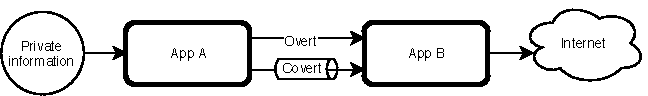
\includegraphics[width=1.0\textwidth]{figures/Collusion1}
	\caption{Structure of a basic app collusion example.}
	\label{fig:sample}
\end{figure}

An early example of this kind of collusion was described by
\citeauthor{Schlegel2011}~\cite{Schlegel2011}\DIFdelbegin \DIFdel{. In their case, in place of the }%DIFDELCMD < \app{A} %%%
\DIFdel{was the Soundcomber}\DIFdelend \DIFaddbegin \DIFadd{, Soundcomber,
that is an }\DIFaddend app that obtained private information using the
microphone. To avoid detection, \DIFdelbegin \DIFdel{the Soundcomber app }\DIFdelend \DIFaddbegin \DIFadd{Soundcomber }\DIFaddend did not have
permission to access the internet, \DIFdelbegin \DIFdel{so }\DIFdelend they proposed to use a
second app to exfiltrate the information. \DIFdelbegin \DIFdel{Similar }\DIFdelend \DIFaddbegin \DIFadd{A similar
}\DIFaddend hypothetical example is also described by
\citeauthor{Asavoae2017}~\cite{Asavoae2017}, where \DIFdelbegin \DIFdel{the }\DIFdelend \DIFaddbegin \DIFadd{one app,
}\DIFaddend \app{A}\DIFaddbegin \DIFadd{, }\DIFaddend would be a contacts app with READ\_CONTACTS
permission, and \DIFdelbegin \DIFdel{the }\DIFdelend \DIFaddbegin \DIFadd{anther app, }\DIFaddend \app{B}\DIFdelbegin \DIFdel{would be }\DIFdelend \DIFaddbegin \DIFadd{, was }\DIFaddend a weather app
with INTERNET permission. However, no such examples have
been reported in the \DIFdelbegin \DIFdel{wild}\DIFdelend \DIFaddbegin \DIFadd{real world}\JWNOTE{Is this true, based on paragraph below?}\DIFaddend .

There is one known example of app collusion in the wild
reported by \citeauthor{Blasco2016}~\cite{Blasco2016}. 
\DIFdelbegin \DIFdel{It is }\DIFdelend \DIFaddbegin \DIFadd{Their analysis revealed }\DIFaddend a set of apps from different vendors
\DIFdelbegin \DIFdel{, all of which included a library known as }\DIFdelend \DIFaddbegin \DIFadd{had a collusion attack. They identified that }\DIFaddend the MoPlus SDK
\DIFdelbegin \DIFdel{. These appswere }\DIFdelend \DIFaddbegin \DIFadd{was common across all of these apps. The collusion attack was }\DIFaddend noticed
after a manual review of apps that were previously labelled
\DIFaddbegin \JWNOTE{Labelled? What does this mean? Need to discuss more of the method I think.}
\DIFaddend as potentially unwanted\DIFaddbegin \JWNOTE{What features would an app have to be ``unwanted''?}\DIFaddend , and were capable of accessing
shared preferences files from different apps. \DIFaddbegin \DIFadd{The }\DIFaddend MoPlus SDK was
already known to contain remote-control capability\DIFdelbegin \DIFdel{, but }\DIFdelend \DIFaddbegin \JWNOTE{Cite?}\DIFadd{, and }\DIFaddend is
now confirmed to also conduct a collusion between different
instances of itself.

\TODO{Add figure depicting the MoPlus SDK}

The MoPlus SDK may be embedded into many different apps,
with 20 such being identified by~\cite{Blasco2016}. \DIFdelbegin \DIFdel{It can then open }\DIFdelend \DIFaddbegin \DIFadd{MoPlus
opens }\DIFaddend a local HTTP server allowing the attacker to abuse
any permissions given to its host app. With potentially many
instances of the MoPlus SDK running on the same device with
different permissions, they would work together to guarantee
that only the instance with highest level of permissions is
the one that starts accepting remote commands. No sensitive
information is exchanged between the apps, but still all
three properties of app collusion are present.


\section{Existing methods for detecting collusions}
\label{sec:approaches}

Attempts with various scopes and outcomes have been made to
detect app collusion. Results range from relatively
computationally easy but very coarse filters to more
accurate but very expensive approaches.
\DIFaddbegin \JWNOTE{This paragraph does not tell me much. We should discuss this.}
\DIFaddend 

\subsection{Based on permissions/interfaces}
\label{sec:filter}

The simplest approach is to base the analysis on statically
extracted features of apps, such as the set of permissions
declared in their manifests\DIFaddbegin \JWNOTE{This is first mention of manifests}
\DIFaddend or the set of Android APIs they import\DIFdelbegin \DIFdel{. This way large amounts of
apps can be quicklyscanned, but necessarily only rough estimations can be made, since very little information about the apps is actually used in }\DIFdelend \DIFaddbegin \JWNOTE{In code? Did this require decompilation of apps? Was any information lost?}\DIFadd{.
Extracting these features from apps allow a large amount of
apps to be quickly}\JWNOTE{Is it quick once you have features? Is it overall a quick process?}
\DIFadd{scanned. The obtained results provide rough estimations of app
collusion, since coarse information about apps is used in the
}\DIFaddend decision making. \DIFdelbegin %DIFDELCMD < 

%DIFDELCMD < %%%
\DIFdel{For example , }\DIFdelend \DIFaddbegin \DIFadd{One example by }\DIFaddend \citeauthor{Asavoae2016}~\cite{Asavoae2016}
\DIFdelbegin \DIFdel{describe }\DIFdelend \DIFaddbegin \DIFadd{describes }\DIFaddend a filtering method based on \DIFaddbegin \DIFadd{an }\DIFaddend app's API calls\DIFaddbegin \DIFadd{, }\DIFaddend and the
permissions declared in its manifest file. \DIFdelbegin \DIFdel{They }\DIFdelend \DIFaddbegin \DIFadd{\mbox{%DIFAUXCMD
\citeauthor{Asavoae2016} }\hspace{0pt}%DIFAUXCMD
}\DIFaddend define
collusion as a pair of apps that satisfy \DIFdelbegin \DIFdel{these }\DIFdelend \DIFaddbegin \DIFadd{the following }\DIFaddend three
conditions:
\DIFdelbegin %DIFDELCMD < \begin{enumerate}
%DIFDELCMD < 	%%%
\DIFdelend %DIF > 
\DIFaddbegin \begin{enumerate}[label=C\arabic*]
	\DIFaddend \item \DIFdelbegin \DIFdel{First }\DIFdelend \DIFaddbegin \DIFadd{One }\DIFaddend app declares a permission that \DIFdelbegin \DIFdel{they classified as giving }\DIFdelend \DIFaddbegin \DIFadd{gives }\DIFaddend access to
	sensitive information.
\DIFaddbegin 

	\DIFaddend \item \DIFdelbegin \DIFdel{Second }\DIFdelend \DIFaddbegin \DIFadd{Another }\DIFaddend app declares a permission that \DIFdelbegin \DIFdel{they classified as giving app the
	ability }\DIFdelend \DIFaddbegin \DIFadd{gives the
	app a permission }\DIFaddend to send information to the outside world.
\DIFaddbegin 

	\DIFaddend \item Finally, \DIFdelbegin \DIFdel{first app }\DIFdelend \DIFaddbegin \DIFadd{both apps }\DIFaddend must be able to send \DIFdelbegin \DIFdel{, and
	second app able to receive}\DIFdelend \DIFaddbegin \DIFadd{and
	receive, respectively, }\DIFaddend on the same channel. They
	\DIFdelbegin \DIFdel{consider the following channels:
	}%DIFDELCMD < \begin{singleitems}
%DIFDELCMD < 		\item %%%
\item%DIFAUXCMD
\DIFdelend \DIFaddbegin \DIFadd{considered }\DIFaddend Intents (each action separately)\DIFdelbegin %DIFDELCMD < \item %%%
\item%DIFAUXCMD
\DIFdel{External storage}%DIFDELCMD < \end{singleitems}
%DIFDELCMD < 	%%%
\DIFdel{(They also consider shared preferences , each file separately, but this is now deprecated : }\DIFdelend \DIFaddbegin \DIFadd{, External storage,
	and shared preferences (now deprecated as discussed in
	}\DIFaddend \Sref{sec:overt})
\end{enumerate}
%DIF > 
It is not clear from their description, but can be assumed,
\DIFdelbegin \DIFdel{that they further }\DIFdelend \DIFaddbegin \DIFadd{whether they }\DIFaddend ignore apps that match both \DIFdelbegin \DIFdel{first and second criteria,
because }\DIFdelend \DIFaddbegin \DIFadd{criterion's C1 and C2,
since }\DIFaddend otherwise their filter would \DIFdelbegin \DIFdel{simply detect any app pairs that can }\DIFdelend \DIFaddbegin \DIFadd{detect any pair of apps
that }\DIFaddend communicate using one of these channels. They
claim that this approach over-approximates\DIFaddbegin \JWNOTE{What does this mean? What if it didn't?} \DIFaddend the set of
colluding apps, while actually it must be noted that they
only consider a narrow subset of app collusions, and, for
example, the MoPlus SDK would be labelled as benign by this
approach.\DIFaddbegin \JWNOTE{Very long sentence. Needs clarification as message isn't coming through.}
\DIFaddend 

\citeauthor{Chen2018}~\cite{Chen2018} propose a similar
approach. \DIFdelbegin \DIFdel{First, they notice that exists }\DIFdelend \DIFaddbegin \DIFadd{They apply }\DIFaddend a machine learning algorithm that \DIFdelbegin \DIFdel{, given
the }\DIFdelend \DIFaddbegin \DIFadd{given
a }\DIFaddend set of all API calls in an app, \DIFaddbegin \DIFadd{it }\DIFaddend can predict whether \DIFdelbegin \DIFdel{the }\DIFdelend \DIFaddbegin \DIFadd{an
}\DIFaddend app is malicious or not. \DIFdelbegin \DIFdel{For communication they only consider intentsas a possible channel}\DIFdelend \DIFaddbegin \DIFadd{Only a single overt channel is captured
for communication between apps, as their work only considers intents}\DIFaddend .
For each app they detect which intents it can send
and receive, and \DIFdelbegin \DIFdel{then they group together apps that }\DIFdelend \DIFaddbegin \DIFadd{they then classify which apps }\DIFaddend could
communicate with each other. \DIFdelbegin \DIFdel{Finally, to detect, whether }\DIFdelend \DIFaddbegin \DIFadd{To perform detection on }\DIFaddend a
group of apps \DIFdelbegin \DIFdel{is }\DIFdelend \DIFaddbegin \DIFadd{to determine if they are }\DIFaddend benign or malicious,
they pass the union of all API calls \DIFdelbegin \DIFdel{of }\DIFdelend \DIFaddbegin \DIFadd{used by }\DIFaddend the apps in the
group to the \DIFdelbegin \DIFdel{aforementioned machine learning algorithm}\DIFdelend \DIFaddbegin \DIFadd{trained machine learning classifier}\DIFaddend .

Neither of these approaches \DIFaddbegin \DIFadd{by \mbox{%DIFAUXCMD
\citeauthor{Asavoae2016} }\hspace{0pt}%DIFAUXCMD
and
\mbox{%DIFAUXCMD
\citeauthor{Chen2018} }\hspace{0pt}%DIFAUXCMD
}\DIFaddend can detect whether apps \DIFdelbegin \DIFdel{actually }\DIFdelend communicate
with each other, nor what kind of information is
exchanged between apps\DIFdelbegin \DIFdel{if they do communicate, since they use no information about }\DIFdelend \DIFaddbegin \DIFadd{. Both methods do not capture }\DIFaddend the
order of \DIFaddbegin \DIFadd{the }\DIFaddend operations within apps. Additionally, they both
consider \DIFdelbegin \DIFdel{only limited }\DIFdelend \DIFaddbegin \DIFadd{a limited set of }\DIFaddend overt channels.

\subsection{Based on control flow analysis}
\label{sec:flow}

A more accurate detection of collusion can be achieved when
the code of apps is also analysed to detect whether or not
they communicate, and what kind of information can they
exchange. Model-based and runtime approaches have been taken
to that.

\citeauthor{Asavoae2018}~\cite{Asavoae2018} describe a
method for checking whether information theft through
collusion exists within the set of possible control flows
for an app. They propose annotating each object returned by
one of predefined Android APIs with the initiating app ID
and a boolean ``sensitive''. Whenever an object is used, its
sensitivity and app ID values are propagated to all
resulting objects. Input set of apps is considered to be
colluding if an object marked sensitive is passed to one of
predefined exporting Android APIs so that the current app ID
is different to the initial app ID from the object. They
explore analysing concrete semantics, in which case the
analysis takes longer, or even forever when the app code
contains any loops, and propose a abstraction of Android app
semantics, which is less accurate, but guaranteed to provide
an answer. They only consider intent based inter-app
communication.

Another approach is to modify the Android \gls{os} to track
information flow at runtime. Example of this is
TaintDroid~\cite{Enck2014}, which can track information
flows from sensitive sources to sensitive sinks system wide,
but incurs a $14\%$ CPU overhead doing so. They use
variable-level label tracking within app code (by augmenting
the Java \gls{vm}), message-level tracking in Binder,
method-level tracking for native system libraries, and
file-level tracking. Therefore, this approach is only
capable of tracking information flow within Java code,
intents, Android API calls, and files, but native code is
not tracked (authors here approached this by banning all
native components in apps, breaking $5\%$ of apps by some
estimates). \todo{limited channels}Use of labels is similar
to~\cite{Asavoae2018}, but amount of false positives is much
smaller, because corresponding exit state must be actually
reached for it to be reported. False negatives may be caused
when labels are not propagated through covert channels, and
false positives when label propagation is overly
conservative.

\subsection{Other}
\label{sec:othermethods}

None of the above approaches have been able to detect
collusion using covert channels. People have looked into
closing some covert channels~\tocite{}, but it is not
reasonable to assume that all covert channels can be found.
Additionally, even today there exist known open covert
channels (\Sref{sec:covert}).

\citeauthor{Muttik2016}~\cite{Muttik2016} proposes
augmenting aforementioned approaches with additional
heuristic rules. He argues that colluding apps can
\todo{order of words}be also detected using indirect
signals, for example whether apps come from the same source,
explicitly encourage co-installation, are frequently
installed together, use similar libraries, etc. Furthermore,
he notes that signals like publication date, app market and
installation method can be used. Finally,
\citeauthor{McAfee2016} also claims to use manual review and
reverse engineering to make final decisions about apps.

Already in 2016 \citeauthor{McAfee2016} claimed that their
product is able to detect colluding mobile apps and stop
them from running~\cite{McAfee2016}. However, based on known
information about the state of the art, this is unlikely to
be entirely true.

\section{Conclusion}
\label{sec:conclusion}

%============================================================

\bibliographystyle{IEEEtranNDoi}
\bibliography{ieee,oro-cs-seminar}

\listoftodos
\TODO{remove list of todos}

\end{document}
